\section{Interpolation on the exponent set}
\label{sec:interpolation}

We prove that the limiting matrix~\eqref{eq:limiting-matrix} has full
column rank when the common multiplicity is sufficiently large at a
fixed ratio $d/m$. The final assembly will achieve that size by taking
a common power. The matrix columns are indexed by the finite exponent set
$\mathcal S$ of~\eqref{eq:exponent-set}, and its rows are the
restrictions to $\mathcal S$ of the monomials
\[
 K^\ell J^b,\qquad 0\le b<m,\quad 0\le\ell<q(m-b),
\]
where evaluation at $(j,K)$ substitutes $J=j$. Thus full column rank
means that their span interpolates every function on $\mathcal S$.
We first give a sufficient condition in terms of the distribution of
horizontal row sizes. We then prove that condition by enclosing
$\mathcal S$ in a polygon and counting its horizontal slices.
All parameters remain fixed as in Section~\ref{sec:elliptic}; in
particular, $q=r-9$ and $h=m\rho>0$.

\subsection{Interpolation by horizontal rows}

The interpolation procedure treats larger rows first and multiplies
each correction by factors vanishing on all previously treated rows.
The number of earlier rows controls the degree in $K$, while the
current row size controls the degree in $J$. Their joint constraint
explains why a bound on the largest row, or on the total number of
points, would not suffice.

\begin{lemma}[Interpolation by horizontal rows]\label{lem:interpolation}
Let $q,m$ be positive integers and $S\subset\C^2$ a finite set,
with coordinates $(j,K)$. For each represented height $K$, let $N_K$
be its row size. Suppose
\[
 N_K\le m,\qquad
 \#\{K:N_K\ge t\}\le q(m-t+1)
 \quad(1\le t\le m,\ t\in\Z).
\]
Then every function $S\to\C$ is the restriction of a polynomial in
\[
 \mathcal P_{q,m}
 =\operatorname{span}_{\C}
 \bigl\{K^\ell J^b:0\le b<m,\quad0\le\ell<q(m-b)\bigr\}
 \subset\C[J,K].
\]
Here evaluation at $(j,K)$ substitutes $J=j$.
\end{lemma}

\begin{proof}
The empty set is immediate. Otherwise order the distinct heights as
$K_1,\ldots,K_s$ so that their sizes $N_1,\ldots,N_s$ are
nonincreasing. The first $i$ rows have size at least $N_i$, even
when sizes are tied, and hence
\begin{equation}\label{eq:ordered-row-bound}
 i\le\#\{K:N_K\ge N_i\}\le q(m-N_i+1).
\end{equation}

Starting with the zero polynomial, match the prescribed values one
row at a time. For row $i$, put
\[
 Q_i(K)=\prod_{a=1}^{i-1}(K-K_a),
\]
where the empty product is one. Since $Q_i(K_i)\ne0$ and the $N_i$
first coordinates on this row are distinct, univariate interpolation
gives a polynomial $p_i(J)$ of degree at most $N_i-1$ such that
$Q_i(K_i)p_i(j)$ is the correction required at every point of row
$i$. Adding $Q_i(K)p_i(J)$ matches that row and preserves all
previous rows.

Every monomial of this correction has $b\le N_i-1<m$ and
\[
 \ell\le i-1<q(m-N_i+1)\le q(m-b),
\]
by~\eqref{eq:ordered-row-bound}. Thus each correction belongs to
$\mathcal P_{q,m}$, and their sum interpolates the prescribed values.
\end{proof}

For the exponent set $\mathcal S$, it remains to prove the two row
bounds in this lemma. We will obtain them by enclosing $\mathcal S$
in a polygon and using its horizontal slice lengths to count the rows.

\subsection{An enclosing polygon}

Write $a=\rho_*=3(\sqrt r-3)>0$, and set
\[
 U_0=\frac h9(a-\Delta)+ma,
 \qquad X=\frac jm,\qquad Y=\frac{K-U_0}{m}.
\]
Thus $U_0$ is the lower endpoint of the exponent interval for $j=0$.
For $0<\lambda\le1$, and with $t_+=\max\{t,0\}$, define
\begin{equation}\label{eq:enclosing-polygon}
 \mathcal D_\lambda
 =\bigl\{(X,Y)\in\mathbb R^2:
 X\ge0,\quad
 -aX\le Y\le-aX+\lambda a-9(X-\lambda)_+\bigr\}.
\end{equation}
By~\eqref{eq:delta}, we have $\rho+\Delta\rho/9<a$. Choose
$0<\lambda<1$ sufficiently close to $1$ that
\begin{equation}\label{eq:lambda}
 \rho+\frac{\Delta\rho}{9}<\lambda a-9(1-\lambda).
\end{equation}
This choice depends only on $r$, the ratio $d/m$, and $\Delta$.
We will show that this inequality places $\mathcal S$ inside
$m\mathcal D_\lambda+(0,U_0)$. The horizontal widths of this
scaled, translated polygon will be at most
$m\lambda<m$, and the heights supporting a slice of length at least
$s$ will form an interval of length $q(m\lambda-s)$ for
$0\le s\le m\lambda$.

\begin{lemma}\label{lem:exponent-enclosure}
Every pair $(j,K)\in\mathcal S$ satisfies
\begin{equation}\label{eq:exponent-polygon}
 \begin{aligned}
 0&\le X\le1+\rho/9,\\
 -aX+\Delta(X-1)_+
 &\le Y\le-aX+\rho+(\Delta-9)(X-1)_+.
 \end{aligned}
\end{equation}
The region in~\eqref{eq:exponent-polygon} is contained in
$\mathcal D_\lambda$. Consequently,
$\mathcal S\subseteq m\mathcal D_\lambda+(0,U_0)$.
\end{lemma}

\begin{proof}
The index bound $j\le\lfloor d/3\rfloor$ gives
$X\le d/(3m)=1+\rho/9$. For $j\le m$, the exponent interval is
\[
 U_0-aj<K<U_0-aj+h,
\]
which gives the first branches of the two bounds. For $j>m$ with
$d-3j>0$, its length is $n=h-9(j-m)$ and its lower endpoint is
$n(a-\Delta)/9$. The identities
\[
 \frac n9(a-\Delta)-U_0=-aj+\Delta(j-m),
 \qquad n=h-9(j-m)
\]
give the second branches after division by $m$.

If a degree-zero block occurs, its sole exponent is
$(j,K)=(d/3,0)$, where $j=m+h/9$. Hence
\[
 X=1+\rho/9,\qquad
 Y=-a-\frac\rho9(a-\Delta).
\]
Both bounds in~\eqref{eq:exponent-polygon} equal this value, so the
endpoint is included.

For containment, the lower bound is at least $-aX$. If $X\le1$,
then~\eqref{eq:lambda} gives
\[
 \lambda a-9(X-\lambda)_+
 \ge\lambda a-9(1-\lambda)>\rho.
\]
If $1\le X\le1+\rho/9$, subtracting the common term
$-aX-9(X-1)$ from the upper bounds reduces their comparison to
\[
 \rho+\Delta(X-1)
 \le\rho+\Delta\rho/9
 <\lambda a-9(1-\lambda),
\]
by~\eqref{eq:lambda}. Thus the entire region, including its
endpoint, lies in $\mathcal D_\lambda$.
\end{proof}

\subsection{Horizontal slices and integer rows}

The length of a bounded interval is the difference of its endpoints;
a singleton has length zero. When a required length is zero, we still
require the slice to be nonempty.

\begin{lemma}[Horizontal slice profile]\label{lem:slice-profile}
We have $\mathcal D_\lambda=\lambda\mathcal D_1$. The nonempty
horizontal slices of $\mathcal D_1$ have lengths
\[
 w(Y)=
 \begin{cases}
  1-Y/a,&0\le Y\le a,\\[1mm]
  1+Y/\bigl(a(1+a/9)\bigr),
       &-a(1+a/9)\le Y\le0.
 \end{cases}
\]
Their maximum length is one. For $0\le s\le m\lambda$, the heights
of nonempty slices of $m\mathcal D_\lambda+(0,U_0)$ of length at
least $s$ form the closed interval
\[
 \bigl[
 U_0-a(1+a/9)(m\lambda-s),\;
 U_0+a(m\lambda-s)
 \bigr],
\]
whose length is $q(m\lambda-s)$.
\end{lemma}

\begin{proof}
Scaling both coordinates by $\lambda$ in~\eqref{eq:enclosing-polygon}
gives $\mathcal D_\lambda=\lambda\mathcal D_1$. The lower boundary
of $\mathcal D_1$ is $Y=-aX$ and its upper boundary is
\[
 Y=\begin{cases}
 a(1-X),&0\le X\le1,\\
 (a+9)(1-X),&X\ge1.
 \end{cases}
\]
Thus its vertices are
\[
 (0,0),\quad(0,a),\quad(1,0),\quad
 \bigl(1+a/9,-a(1+a/9)\bigr).
\]
The slices are
\[
 \begin{array}{ll}
 0\le X\le1-Y/a,&0\le Y\le a,\\[1mm]
 -Y/a\le X\le1-Y/(a+9),&-a(1+a/9)\le Y\le0,
 \end{array}
\]
and are empty at all other heights. Their lengths are the stated
functions, since
$1+Y/a-Y/(a+9)=1+Y/\bigl(a(1+a/9)\bigr)$.
Both attain their maximum one at $Y=0$.

Scale by $m\lambda$ and translate vertically by $U_0$. Solving
these two linear inequalities for length at least $s$ gives the
claimed closed interval. Its length is
\[
 (2a+a^2/9)(m\lambda-s)=q(m\lambda-s),
\]
because $a=3(\sqrt r-3)$ implies $2a+a^2/9=r-9=q$.
At $s=m\lambda$ the interval is the single height $U_0$; at $s=0$
it is the full vertical range of the polygon.
\end{proof}

\begin{figure}[htbp]
 \centering
 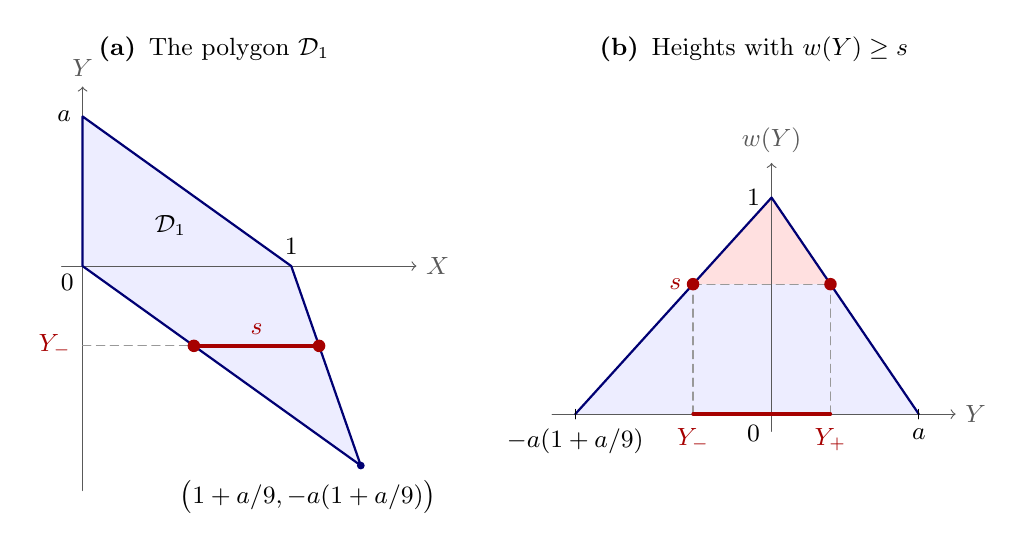
\begin{tikzpicture}[
  font=\small,
  line cap=round,
  line join=round,
  axis/.style={->,thin,black!65},
  boundary/.style={thick,blue!45!black},
  guide/.style={densely dashed,thin,black!40},
  sample/.style={very thick,red!65!black},
  slicepoint/.style={circle,inner sep=1.6pt,fill=red!65!black}
]
  \begin{scope}[x=2.65cm,y=1.90cm]
    \node[anchor=south] at (.63,1.30)
      {\textbf{(a)}\enspace The polygon $\mathcal D_1$};
    \fill[blue!7] (0,0)--(0,1)--(1,0)--(4/3,-4/3)--cycle;
    \draw[axis] (-.10,0)--(1.60,0) node[right] {$X$};
    \draw[axis] (0,-1.50)--(0,1.20) node[above] {$Y$};
    \draw[boundary] (0,0)--(0,1)--(1,0)--(4/3,-4/3)--cycle;
    \node[anchor=south west] at (.30,.14) {$\mathcal D_1$};
    \node[anchor=north east,inner sep=3pt] at (0,0) {$0$};
    \node[anchor=east,inner sep=4pt] at (0,1) {$a$};
    \node[anchor=south,inner sep=4pt] at (1,0) {$1$};
    \draw[guide] (0,-8/15)--(8/15,-8/15);
    \draw[sample] (8/15,-8/15)--(17/15,-8/15);
    \node[slicepoint] at (8/15,-8/15) {};
    \node[slicepoint] at (17/15,-8/15) {};
    \node[anchor=east,inner sep=4pt,text=red!65!black]
      at (0,-8/15) {$Y_-$};
    \node[anchor=south,inner sep=4pt,text=red!65!black]
      at (5/6,-8/15) {$s$};
    \fill[blue!45!black] (4/3,-4/3) circle (1.4pt);
    \node[anchor=north,inner sep=5pt] at (1.08,-4/3)
      {$\bigl(1+a/9,-a(1+a/9)\bigr)$};
  \end{scope}

  \begin{scope}[shift={(8.75cm,-1.88cm)},x=1.87cm,y=2.75cm]
    \node[anchor=south] at (-.12,1.58)
      {\textbf{(b)}\enspace Heights with $w(Y)\ge s$};
    \fill[blue!7] (-4/3,0)--(0,1)--(1,0)--cycle;
    \fill[red!12] (-8/15,3/5)--(0,1)--(2/5,3/5)--cycle;
    \draw[axis] (-1.49,0)--(1.25,0) node[right] {$Y$};
    \draw[axis] (0,-.08)--(0,1.16) node[above] {$w(Y)$};
    \draw[boundary] (-4/3,0)--(0,1)--(1,0);
    \draw[guide] (-8/15,0)--(-8/15,3/5);
    \draw[guide] (2/5,0)--(2/5,3/5);
    \draw[guide] (-8/15,3/5)--(2/5,3/5);
    \draw[sample] (-8/15,0)--(2/5,0);
    \node[slicepoint] at (-8/15,3/5) {};
    \node[slicepoint] at (2/5,3/5) {};
    \draw[thin] (-4/3,.022)--(-4/3,-.022);
    \draw[thin] (1,.022)--(1,-.022);
    \node[anchor=north,inner sep=5pt] at (-4/3,0)
      {$-a(1+a/9)$};
    \node[anchor=north,inner sep=5pt] at (1,0) {$a$};
    \node[anchor=north east,inner sep=4pt] at (0,0) {$0$};
    \node[anchor=east,inner sep=4pt] at (0,1) {$1$};
    \node[anchor=north,inner sep=5pt,text=red!65!black]
      at (-8/15,0) {$Y_-$};
    \node[anchor=north,inner sep=5pt,text=red!65!black]
      at (2/5,0) {$Y_+$};
    \node[anchor=east,inner sep=4pt,text=red!65!black]
      at (-8/15,3/5) {$s$};
  \end{scope}
\end{tikzpicture}

 \caption{Slice widths and their superlevel interval for
 $\mathcal D_1$, drawn schematically with $a=\rho_*$ and
 $0<s<1$. In panel~(a), the marked slice at
 $Y_-=-a(1+a/9)(1-s)$ has length $s$. In panel~(b), slices of
 length at least $s$ occur exactly at heights from $Y_-$ to
 $Y_+=a(1-s)$, an interval of length $q(1-s)$.
 Scaling by $m\lambda$ and translating by $(0,U_0)$ gives the
 polygon and height intervals used to bound the integer rows.}
 \label{fig:slice-profile}
\end{figure}

For each integer $K$, let
\[
 N_K=\#\{j\in\Z:(j,K)\in\mathcal S\}.
\]
Only finitely many of these row sizes are nonzero. The slice profile
in Figure~\ref{fig:slice-profile} bounds both each row size and the
number of rows of any given minimum size.
The passage from lengths to integer counts adds at most one endpoint.
We will absorb it with the size condition
\begin{equation}\label{eq:scaling}
 q(1-\lambda)m\ge1.
\end{equation}

\begin{lemma}[Integer row counts]\label{lem:integer-rows}
If $q(1-\lambda)m\ge1$, then the exponent set satisfies
\begin{equation}\label{eq:row-count}
 \begin{aligned}
 N_K&\le m &&(K\in\Z),\\
 \#\{K\in\Z:N_K\ge t\}
 &\le q(m-t+1) &&(1\le t\le m,\ t\in\Z).
 \end{aligned}
\end{equation}
\end{lemma}

\begin{proof}
By Lemmas~\ref{lem:exponent-enclosure} and~\ref{lem:slice-profile},
the integer positions in a represented row lie in an interval of
length at most $m\lambda<m$. Their span is at least $N_K-1$, so
integrality gives $N_K\le m$, also for a singleton row.

A row with $N_K\ge t$ requires a nonempty slice of length at least
$t-1$. If $t-1>m\lambda$, there are no such rows. Otherwise their
integer heights lie in a closed interval of length
$q(m\lambda-t+1)$. An interval of length $L\ge0$ contains at most
$\lfloor L\rfloor+1\le L+1$ integers. Therefore
\[
 \begin{aligned}
 \#\{K\in\Z:N_K\ge t\}
 &\le q(m\lambda-t+1)+1\\
 &=q(m-t+1)-q(1-\lambda)m+1\\
 &\le q(m-t+1)
 \end{aligned}
\]
by~\eqref{eq:scaling}. The extra one accounts for integral endpoints,
including when the height interval is a singleton.
\end{proof}

\subsection{Full rank and the strict inequality}

\begin{proposition}\label{prop:full-rank}
If $q(1-\lambda)m\ge1$, then the limiting matrix $B_0$
of~\eqref{eq:limiting-matrix} has full column rank. Consequently,
$J_\tau$ is injective for all sufficiently small positive $\tau$.
\end{proposition}

\begin{proof}
Apply Lemma~\ref{lem:interpolation} to $S=\mathcal S$, using
Lemma~\ref{lem:integer-rows}. The row vectors of $B_0$ are the
restrictions to $\mathcal S$ of the monomials spanning
$\mathcal P_{q,m}$. They therefore span $\C^{\mathcal S}$, so
$B_0$ has rank $\#\mathcal S$. Proposition~\ref{prop:matrix-limit}
then gives the injectivity of $J_\tau$ for sufficiently small $\tau$.
\end{proof}

\begin{proof}[Completion of the proof of Theorem~\ref{thm:main}]
By Lemma~\ref{lem:universal}, it suffices to exclude every universal
system $\mathsf U_r(d,m)$ with $d/m\le\sqrt r$.
Proposition~\ref{prop:squares} does so when $r$ is a square,
including equality.

For nonsquare $r$, the rational ratio $d/m$ is strictly below
$\sqrt r$, and Lemma~\ref{lem:cubic-low-degree} forces $d/m>3$.
Choose $\Delta$ as in~\eqref{eq:delta} and $\lambda$ as
in~\eqref{eq:lambda}. By Lemma~\ref{lem:universal}, replace
$(d,m)$ by a common positive integral multiple large enough to
satisfy~\eqref{eq:scaling}. The ratio $d/m$, and hence the choices
of $\rho$, $\Delta$, and $\lambda$, do not change. Apply all the
preceding constructions to this one chosen pair. Then
Proposition~\ref{prop:necessary-W} and Lemma~\ref{lem:collision}
give a nonzero kernel of $J_\tau$ for every fixed $\tau\in(0,1)$.
Proposition~\ref{prop:full-rank} gives an injective $J_\tau$ for
all sufficiently small positive $\tau$, a contradiction. The collision
has been taken on each fixed curve before the matrix limit; no
simultaneous choice of kernel vectors is needed.

There are therefore no universal systems of the required slope.
Lemma~\ref{lem:universal} supplies the single countable union $E_r$
and the strict inequality outside it, simultaneously for every
positive degree and every nonnegative integral multiplicity vector.
That reduction concerns all nonzero homogeneous forms, so the
conclusion includes reducible and nonreduced effective curves.
\end{proof}
